\documentclass[pdftex,12pt,a4paper]{article}

\usepackage{graphicx}
\DeclareGraphicsExtensions{.jpg}
\usepackage{float}
\usepackage[labelfont=bf]{caption}

\frenchspacing

\newcommand{\HRule}{\rule{\linewidth}{0.5mm}}

\begin{document}
\begin{titlepage}
\begin{center}

%Title
\HRule \\[0.5cm]
{\huge \bfseries HVD-1\\[0.5cm]}
\HRule \\[1.0cm]

\textsc{\LARGE HDMI Video Divider ver 1.0}\\
[1.5cm]

%Engineers
\begin{minipage}{0.9\textwidth}
\begin{flushleft} \large
{\bfseries Engineer:}\\
\emph{Cassandra \textsc{Chow}}
\end{flushleft}
\end{minipage}
%Instructors
\begin{minipage}{0.9\textwidth}
\begin{flushright} \large
{\bfseries Instructors:}\\
\emph{Lukas \textsc{van Ginneken}}

\emph{Jeremy \textsc{Thomas}}

\emph{Christopher \textsc{Theriault}}
\end{flushright}
\end{minipage}

\vfill

%Bottom of Page
{\large DigiPen Institute of Technology}\\
{\large Department of Computer Engineering}\\
{\large ECE 310L, Fall 2014}\\
{\large Revision: 1.0}

\end{center}
\end{titlepage}

\pagebreak
\tableofcontents
\pagebreak

%ABSTRACT
\section{Abstract}
The HVD is designed to duplicate or spatially divide display data from any HDMI signal. The hardware requirements of the HVD and image processing required by the device design will benefit from the parallel processing offered by an FPGA platform\cite{TechDoc_FPGA_Benefits}.  Specifically, the HVD will be implemented with the Cyclone IV on the DE2-115 development board paired with HDMI interface solutions offered by Analog Devices\cite{DataSheet_ADV7611, DataSheet_ADV7513, Guide_ADV7611, Guide_ADV7513}. Development concerning the design and testing of the HDMI interface PCBs and I$^2$C communication will be covered by this paper. Due to the project goals remaining unachieved, evaluation concerning design progress and future planning is also presented. 

%INTRODUCTION
\section{Introduction}

\paragraph{}
As a student we have found FPGA development and communication protocols subject of our highest interests. FPGA devices can enable engineers to use hardware to implement software applications with less concern about application specific device processing constraints. FPGA's reconfigurablility provide system flexibility and adaptability during the design phase. They have no operating system system and use parallel processing paths, giving the designer control of the architecture for processing logic \cite{TechDoc_FPGA_Benefits}.

\paragraph{}
Communication protocols are a means of communicating data between two systems or to device peripherals. The protocols are standardized meaning peripheral devices can communicate with a variety of systems. Communication protocol are essential for several computer system and can vastly improve data processing. Advancements in display protocols in particular has refined how users observe video data. HDMI 2.0, for example, increased video resolution from 1080p to 2160p \cite{Web_HDMI_2.0}. Consumers can enjoy higher resolution images and higher video refresh rates partially due to improvements in protocols. Thus protocols can serve a pivotol role in technological advancement. 

\paragraph{}
With respect to our subjects of interest, FPGA development and protocols, we prepared a design for an FPGA device that primarily relies of communication protocol implementation. This device we came to call the HVD for HDMI Video Divider.As the name suggests, the device's end use will be to spatially divide an HDMI video frame and process each division for output. The HVD will be especially suited for split screen applications. The device implementation  consists of the base FPGA platform, HDMI interface, and I$^2$C driven system intercommunication. This document will overview the system design in detail, procedures used to test the system, and analyze the progress of the device's development within the first development cycle.

%END USER APPLICATION
\section{End User Application}

\paragraph{}
The HVD shall function given standard HDMI display data from any source. This flexibility allows the device implementation opportunities in various applications. Any other HDMI output capable product, such as a DVD player, computer, or video game console, will provide dual video data with the assitance of the HVD. The HVD will exist between the source and display mediums in an application setup. The source HDMI signal will enter the HVD device to be interpreted and optionally divided before duplicated display data or divided display data is sent to respective display mediums. Figure~\ref{fig:use} is a diagram of the theoretical HVD setup for a display divided across two mediums.

% FIGURE
\begin{figure}[H]
\centering
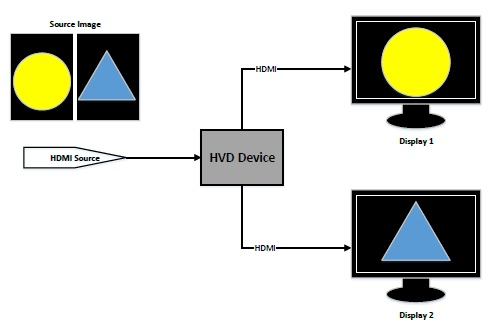
\includegraphics{UserModel.jpg}
\caption{\textbf{Setup for dividing video across two display mediums using the HVD device}}
\label{fig:use}
\end{figure}

\paragraph{}
While the HVD can apply to an arbitrary HDMI source, the suitable applications for this device are more situational. For example, clients wouldn't have any need to divide a movie display across two TVs which may result in decreased video quality. All video applications do not benefit from the features the HVD offers, but several cases do. A split screen application has more obvious use for the HVD. Split screen  is a video technique in which the frames are spatially divided into discrete nonoverlapping images. Cooperative or comptetitve multiplayer video game applications can use this technique to incorporate multi-user designs. However, the nature of such a design allows players to 'screen peek,' a tactic where players might watch an opponent's screen to gain an unfair advantage. With the HVD, this situation can be prevented. Each user's portion of the display can be output to a separate video medium which can be moved to make the display more private to one of the users.

%SYSTEMS DESIGN
\section{Systems Design}

\paragraph{}
The HVD device requires the integration of several systems to provide complete functionality of the necessary features. This section cover the individual design and implementation of each of the HVD's major systems including the system platform, hdmi interface, and I$^2$C communications. Figure~\ref{fig:block} at the end of this section is a block diagram of the entire HVD system design.

%	FPGA PLATFORM
\subsection{FPGA Platform}

\paragraph{}
The Altera DE2-115 Development Board was selected as HVD's processing platform. Implementing the HVD on an FPGA was a easier design solution as opposed to finding an ASIC development solution that matched all the design constraints. These design constraints include support for three HDMI ports and high speed video processing. An FPGA design is suitable for the HVD's design because the highly parallel architecture they offer meet the HDMI performance requirements\cite{TechDoc_FPGA_Benefits}. The DE2-115 digital logic is programmed using the Verilog hardware descriptive language compiled and developed with Altera's toolchain, Quartus II. 

\paragraph{}
Using the DE2-115 ensures we can implement a solution for the HVD design requirements. The on-board 50 MHz clock and PLL clock generator enables the FPGA to process the high speed HDMI . The board does have SDRAM and SRAM, but these memory implementations have insufficient bandwidth to store the data fast enough\cite{UserManual_DE2}. Therefore, we will store data using the Cyclone IV FPGA embedded memory M9K blocks. The M9K blocks features configurable data width and dual-port modes necessary for storing pixel data at the required speeds\cite{TechDoc_M9K}. The HDMI protocol support a pixel clock up to 165 MHz at a resolution of 24 bits per pixel, resulting in the necessity to simultaneously read and write data at almost 4 Gbps\cite{TechDoc_HDMI_Spec}.

\paragraph{}
While the DE2-115 does not provide an HDMI interface solution, the HSMC is a high-speed header that can provide a sufficient amount of GPIO lines to the Cyclone IV for our own integration of an HDMI interface. Paired with the a Terasic GPIO Daughter Board, we HSMC connects to three more GPIO headers\cite{UserManual_THDB-HTG} which can be used to communicate with three HDMI interfaces.

%	HDMI Interface
\subsection{HDMI Interface}

\paragraph{}
The HDMI interface will be implemented using Analog Devices chip solutions. The ADV7611 implements HDMI receiving interface while two ADV7615 will implement each HDMI transmission interface. The HDMI receiver interface translates the differential signals from an HDMI source into 24 parallel pixel data signals\cite{DataSheet_ADV7611}. Audio data is also provided and interpreted by the HDMI interface but is not being implemented in HVD version 1.0. The transmitter interfaces translates 24 parallel pixel data lines into differential signals\cite{DataSheet_ADV7513}. The chips are configured through their main I$^2$V ports which control registers and protocol data such as the info frame or extended display identification data, EDID. Protocol information is essential for identifying and controlling the HDMI configuration of the source device\cite{TechDoc_HDMI_Spec}.

%	SYSTEM COMMUNICATIONS
\subsection{Communications}

\paragraph{}
The DE2-115 must establish communication with the HDMI interfaces. There will be an I$^2$C protocol port generated using the FPGA's digital logic for each interface. The logic of the Verilog module for the I$^2$C protocol is implemented using a finite state machine architecture. The I$^2$C module generates the protocol's serial clock of approximately 390 KHz from the 50 MHz main clock on the DE2-115. The module's logic is handled in two major blocks functioning off of a logic clock and serial clock. State machine transition and serial data is processed on the logic clock while serial clock ticks and byte transaction and processed on the serial clock. The logic and serial clock are generated so that a logic process step will execute between each serial clock cycle so that the data line is correctly set before the serial clock indicates data is valid on the bus. Figure~\ref{fig:sm} shows the state diagram for the I$^2$C module. Both logic block functionality are dependent on this state machine.

% FIGURE
\begin{figure}[H]
\centering
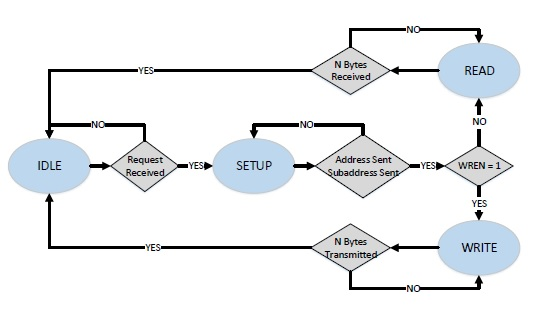
\includegraphics{I2C_SM.jpg}
\caption{\textbf{I$^2$C module finite state machine}}
\label{fig:sm}
\end{figure}

\paragraph{}
The Cyclone IV FPGA acts as the master in the I$^2$C protocol while each register map on the HDMI interfaces are slaves. Since each HDMI interface will have its own dedicated I$^2$C port we can assume the default slave address configurations on each interface.  Each slave device is accessed with a 7-bit address, a R/W bit indicating the nature of the transaction, and an 8-bit sub-address within the register map. The read and write procedures for the HDMI receiver are depicted in Figure~\ref{fig:i2c}\cite{Guide_ADV7611}. The HDMI transmitter is programmed via I$^2$C in the same manner with different register maps.

% FIGURE
\begin{figure}[H]
\centering
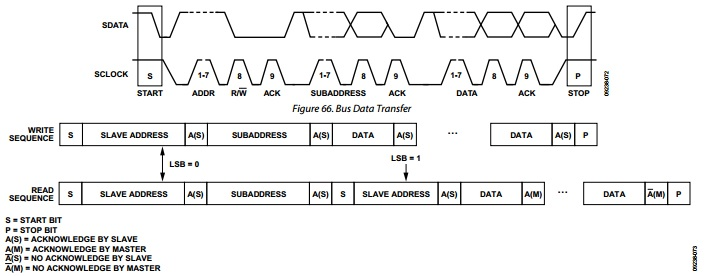
\includegraphics[width=\textwidth]{i2c_rw.jpg}
\caption{\textbf{I$^2$C read and write sequence and bus data signaling. An ACK is indicated by pulling the SDATA line low and a NACK is indicated by pulling the SDATA line high.}}
\label{fig:i2c}
\end{figure}

%	PCB INTEGRATION
\subsection{PCB Integration}

\paragraph{}
To integrate the HDMI interfaces with the DE2-115 the HDMI chips must be housed on a PCB to interface with small chip package. Each HDMI interface PCB will connect to the DE2-115 through a GPIO header on the HSMC to GPIO daughter board. Eagle schematics for the HDMI receiver PCB are located in hdmi\_receiver.sch. Care was taken to include several termination resistors and decoupling capacitors in order to maintain the interface system stability. A 3-layer PCB was design with an internal GND plane and percautions were taken to keep the HDMI differential signals parallel and similar in length. The HDMI transmitter PCBs will have a similar design to the HDMI receiver PCB. Having separate PCB designs for the transmitter and receivers provides individual control over each interface and may simplify component upkeep with separated designs.

%	BLOCK DIAGRAM
\subsection{Block Diagram}

% FIGURE
\begin{figure}[H]
\centering
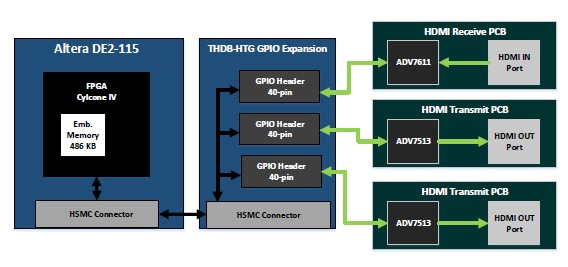
\includegraphics{BlockDiagram.jpg}
\caption{\textbf{HVD systems block diagram}}
\label{fig:block}
\end{figure}

%RESULTS
\section{Results}

%	TIMELINE
\subsection{Timeline}

The past development cycle for the HVD is illustrated in the timeline in Figure~\ref{fig:time}.

% FIGURE
\begin{figure}[H]
\centering
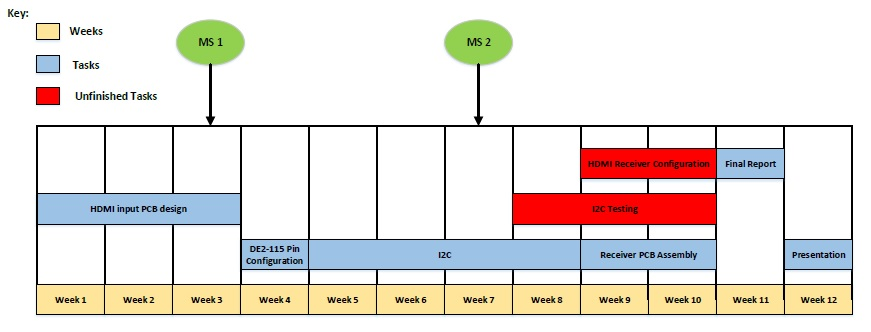
\includegraphics[width=\textwidth]{timeline_fall.jpg}
\caption{\textbf{Development timeline}}
\label{fig:time}
\end{figure}

%	HDMI RECEIVE INTERFACE
\subsection{HDMI Receive Interface}

\paragraph{}
This development cycle focused on the HDMI receive interface implementation including the PCB design, testing, and DE2-115 I$^2$C communication. The receiver was developed first in order to avoid unnecessary development requirements to test the HDMI interface. Ideally to test the HDMI transmit functionality we would ultimately want to transmit a video frame. Instead of having the FPGA generate a video frame, establish a the receiver to acquire a frame instead for later output reduced the software development.

\paragraph{}
The eagle design files for the HDMI receiver PCB are hdmi\_receiver.sch and hdmi\_receiver.brd. This prototype serve as a sufficient test board for identifying early design errors. One such error was already discovered; the footprint for the DC power jack is incorrect making the barrel receptacle impossible to solder to the board without modifications. Further testing is required to verify the functionality of this board which wasn't achieved during this development cycle.

%	I2C PROTOCOL
\subsection{I$^2$C Protocol}
The I$^2$C protocol is essential for controlling the HDMI receive interface using the DE2-115. The I$^2$C module was implemented in Verilog and tested through several mediums. First, Alter'a ModelSim IDE was used to verify the module could be instantiated and successfully produce the desired waveforms in simulation. The real signal generation of the module was observed and checked using oscilloscopes. Some oscilloscope waveform samples are shown and described in Figures~\ref{fig:osc_tx} and~\ref{fig:osc_rx}. This also verified that the pin configurations over the HSMC to GPIO daughter board were correct and functional. Finally, Link Instruments MSO-19.2 with a built in I$^2$C protocol interpreter was used to confirm the I$^2$C module signals were successfully interpreted to comply to the I$^2$C standard. 

% FIGURE
\begin{figure}[H]
\centering
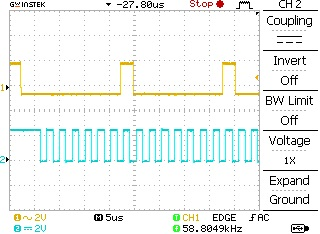
\includegraphics{osc_transmit.jpg}
\caption{\textbf{Screen captured from oscilloscope reading I$^2$C data. The top signal is the SDA and the bottom is SCL.A write sequence is depicted in the captured image. First the SDA is pulled low while the SCL signal is high to indicate a START condition. This enable the generated of the I$^2$C serial clock signal which SCL is connected to. The first data transmitted across the SDA line is the slave address, which in this case is 0x1 in 7-bits. After the 7th bit is transmitted the R/W bit which is zero for a write sequence is sent. On 9th the SCL clock pulse, the SDA line is set to high impedance to acquire an acknowledge input from the slave device. In this case, there is no slave device connected so the SDA remains unchanged. Afterward the subaddress 0x4 is sent in 8-bits in the same fashion. }}
\label{fig:osc_tx}
\end{figure}

% FIGURE
\begin{figure}[H]
\centering
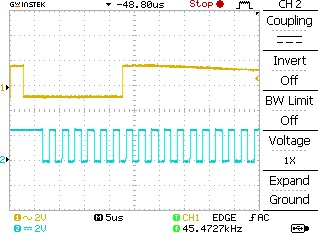
\includegraphics{osc_receive.jpg}
\caption{\textbf{Screen captured from oscilloscope reading I$^2$C data. The top signal is the SDA and the bottom is SCL.A read sequence is depicted in the captured image. Before a read transaction, the subaddress pointer must be set by a previous write transaction. First the SDA is pulled low while the SCL signal is high to indicate a START condition. The first data transmitted across the SDA line is the slave address, which in this case is 0x1 in 7-bits. After the 7th bit is transmitted the R/W bit which is one for a read sequence is sent. ON the 9th SCL clock pulse, the SDA line is set to high impedance to acquire an acknowledge input from the slave deivce. In this case, there is no slave device connected so the SDA remains mostly unchanged. Afterwards the SDA remains set to high impedance to accept input on the SDA line. The SDA line is then only controlled by the master when asserting an ACK or NACK. This signal receives no input but because the SDA line is left at high impedance there is a noticeable decay in the signal. }}
\label{fig:osc_rx}
\end{figure}

\paragraph{}
The simulation and oscilloscope tests and check were successful but the test data offered by the MSO-19.2 gave questionable data that didn't completely confirm our I$^2$C module conformity to the standard protocol. A lack of explicit documentation on the data presented by the I$^2$C interpreter user interface, incorrect signal timing values, and some unexpected protocol behavior makes it so the test in not a perfect verification of the I$^2$C protocol correctness. A sample of MSO-19.2 data is shown and described in Figure~\ref{fig:mso}.

% FIGURE
\begin{figure}[H]
\centering
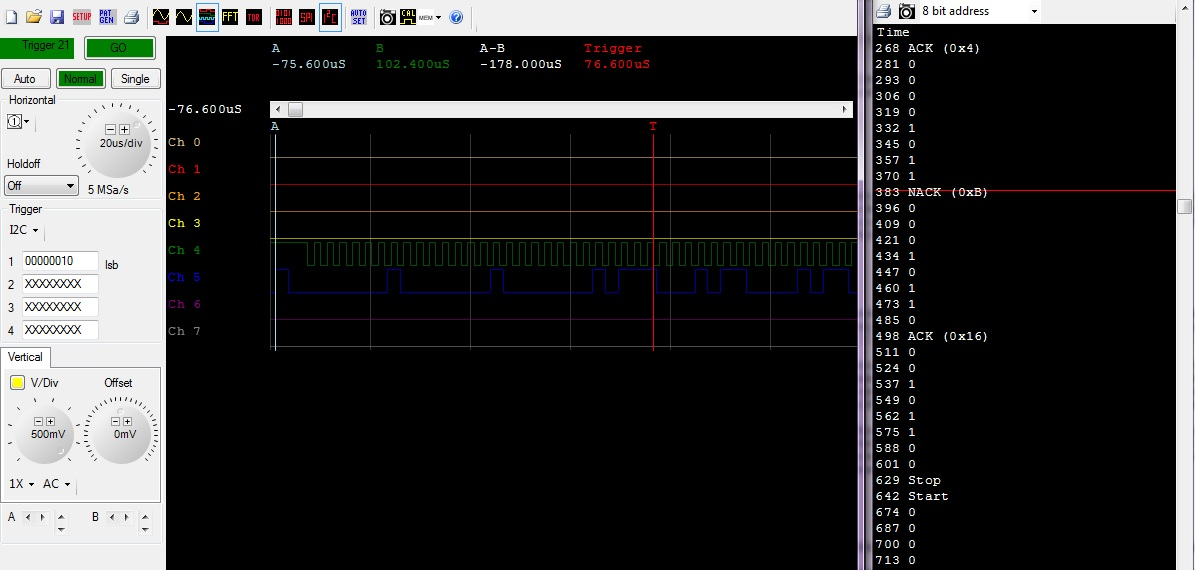
\includegraphics[width=\textwidth]{mso.jpg}
\caption{\textbf{This is MSO data from an I$^2$C write sequence. Channel 4 is the SCL signal and Channel 5 is the SDA signal. The I$^2$C interpreted data is shown in a console window to the right. Start and Stop condition are detected successfully. The data bytes represented in the console window are also correct. However the timing units in microseconds are for some reason off by a factor of 10. Each clock cycle should take approximately 2.5 microseconds while the MSO data shows approximately 25 microseconds. There also is a matter concerning the NACK. The MSO interpeter should generate acknowledge signal for valid I$^2$C data but after receiving a 0xB data byte in this case it generated a NACK. The cause for this is unknown. }}
\label{fig:mso}
\end{figure}

%ANALYSIS
\section{Analysis}

%	TESTING
\subsection{Testing}

\paragraph{}
The HDMI receiver PCB and I$^2$C protocol tests are largely incomplete. The goal for integrated these two systems was also not achieved. Some lack of development foresight in development time led to delays and deviation from the original time line became inevitable. Since the I$^2$C protocol correctness isn't completely verified, we will have to examine if its current implementation is able to properly communicate with the HDMI receive PCB. Examining the functionality of the PCB, ADV7611 HDMI receiver, and the correctness of the I$^2$C protocol at the same time can lead to difficult debugging scenarios involving multiple variables. Unless more investment is made to further test the I$^2$C protocol with additional testing hardware, the cluttered testing scenario may be inevitable.

%	DEVELOPMENT TIME
\subsection{Development Time}

\paragraph{}
Setbacks in the initial development cycle will propagate through to the next. Expected project goals must be re-evaluated. It is an end design goal to be able to process and divide a single HDMI signal into two separate signals. In order to fully implement the hardware and integrate the system, time to development image processing requirements may be sacrificed. The image processing logic, while it is an essential part of the HVD's ideal application, must be the first feature to be dropped from expected implementations in the next development cycle because it reliant on functioning hardware and complete system integration. A proposed time line for next development cycle is shown in Figure~\ref{fig:newtime}. Notice that there is no time reserved for the image processing algorithms necessary for the HVD goal application.

% FIGURE
\begin{figure}[H]
\centering
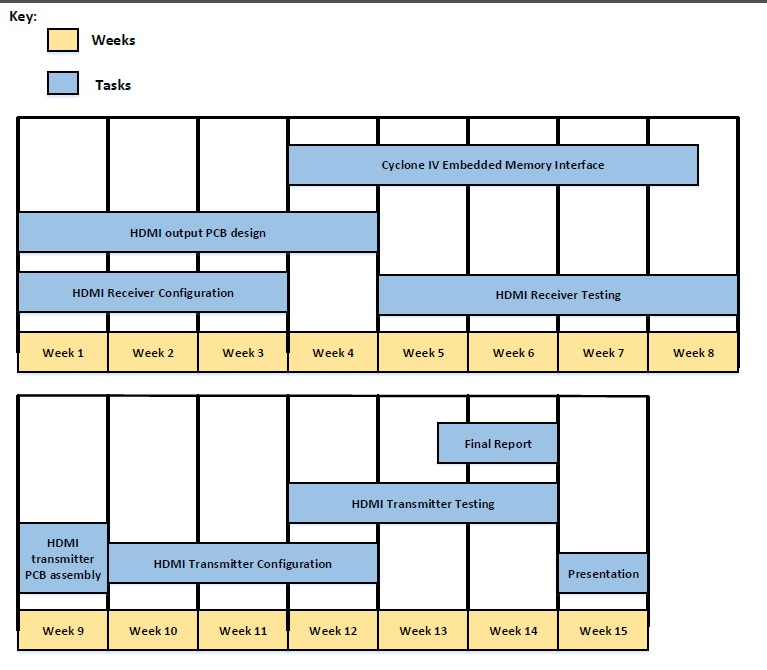
\includegraphics[width=\textwidth]{timeline_spring.jpg}
\caption{\textbf{Next cycle development timeline}}
\label{fig:newtime}
\end{figure}

%	BUDGET
\subsection{Budget}

\paragraph{}
The cost reports for this development cycle was rather high. The PCB fabrication expense for HDMI receiver consumed most of the allowed budget. In order to improve the HVD cost efficiency, future versions should be reduced from a 3-layer to 2-layer board. This will present more design constraints in order to ensure signal integrity. Examining current design faults in the HDMI receive PCB will lend insight when designing the HDMI transmit PCB.

%CONCLUSION
\section{Conclusion}

\paragraph{}
Results of this development cycle are less than optimal. Several pivitol tasks and goals that were not completely satisfied and others were pushed back resulting. However, steady though unideal progress on the development of the HVD systems has deviated little from the original implementation designs. We are confident that the design plans for the HVD remains sound.

\paragraph{}
Overall, the major systems that were suppose to be complete within this cycle still need to be verified and tested. Once all the issues are determined, they can be addressed in future design iterations. While development on the HDMI transmit interface was never achieved, it's similarity to the HDMI receive interface means and problems encountered in devloping the receiver can be avoided when designing the transmitter. The I$^2$C protocol module on the DE2-115 will also function in communication with the transmitter. 

\paragraph{}
In the following cycle, once the previous tasks are completed. A quick rework of the receiver PCB, prototype of the transmitter PCB and I$^2$C integration should be achievable. The remaining time can be spent working on the HDMI configuration software and memory logic on the Cyclone IV. The image processing development has been delayed, but focus on the HVD hardware and interface systems is an absolute priority.

\pagebreak
%ACKNOWLEDGEMENTS
\section{Acknowledgements}

\paragraph{}
We would like to acknowledge the following persons, whose contributions and guidance made the development and execution of this project possible.
\newline
\newline
Lukas van Ginneken for instructing and assisting in planning the project, identifying design constraints, and providing development solutions. Jeremy Thomas for instructing, offering guidance on engineering practices, and encouragement that helped keep us motivated. Christopher Theriault for managing the project budget, acquiring necessary resources, and providing test tools. Nicholas Rivera for sharing his experience and knowledge in embedded systems designs. And Johnny Sim for sharing his experience and knowledge of Altera's FPGA development software.
\newline
\newline
Thank you for all of your support.

%References
\bibliographystyle{ieeetr}
\bibliography{Citation}

\end{document}

